\documentclass[10pt,letterpaper]{article}
\usepackage{neverhuman-brief-style}

\renewcommand{\briefrunningtitle}{Executive Brief}
\title{NEVERHUMAN Pre-Incision POAF Executive Brief}
\author{NEVERHUMAN Research \& HonorHealth Heart Care}

\begin{document}
\thispagestyle{briefpage1}

\briefmasthead{Executive Brief \textbar{} For Health-System CEOs, CMOs \& Chief AI Officers}%
  {Outperform Frontier AI on Unseen Hospitals --- At 117\x{}--323\x{} Faster Speed}%
  {Auditing \textbf{368,132 U.S.\ cardiac surgeries across 1,091 STS centers}, we benchmark five leading binary tabular AI platforms---Google TabFM, NVIDIA Kumo, PriorLabs TabPFN-3.5, CatBoost, and AutoGluon---directly against \textbf{NEVERHUMAN} across strictly unseen and in-network hospitals.}

% ---- 4 KPI Cards ------------------------------------------------------------
\noindent
\begin{minipage}[t]{0.238\textwidth}\vspace{0pt}
\kpicard{navy}{368,132}{National CABG Cases}{Audited across \textbf{1,091 U.S.\ centers}; 24.30\% POAF (89,337 events); strictly 207 pre-incision EHR variables.}
\end{minipage}\hfill
\begin{minipage}[t]{0.238\textwidth}\vspace{0pt}
\kpicard{accent}{0.6767 / 0.7014}{Unseen / In-Net AUC}{\textbf{\#1 at 50k} on 74 unseen hospitals (beats all 5 binary AI models, CI $>0$); seen + EB reaches 0.697--0.701.}
\end{minipage}\hfill
\begin{minipage}[t]{0.238\textwidth}\vspace{0pt}
\kpicard{teal}{4.11\,s (0.19\,ms/pt)}{21,241-Patient Infer}{\textbf{19.7\x{} faster} than AutoGluon (81\,s) \& \textbf{117\x{}--323\x{} faster} than Kumo, TabPFN-3.5 \& TabFM (0.53\,GB VRAM).}
\end{minipage}\hfill
\begin{minipage}[t]{0.238\textwidth}\vspace{0pt}
\kpicard{blue}{20.4--33.8}{Avoided / 100 Patients}{Decision Curve Net Benefit across 25\%--35\% thresholds ($P{>}0{=}1.000$ vs.\ POAF score); \textbf{7.4\x{}} decile spread.}
\end{minipage}

\vspace{4.5pt}

% ---- Executive Narrative (Two Columns) --------------------------------------
\noindent
\begin{minipage}[t]{0.486\textwidth}
  \vspace{0pt}
  \colheading{Why Hospital Validation Splits \& Speed Decide Reality}
  {\fontsize{7.95}{9.95}\selectfont
  Postoperative atrial fibrillation (POAF) complicates \textbf{nearly 1 in 4} isolated CABG surgeries---driving stroke, prolonged ICU stay, and readmissions. High-impact prophylaxis (such as posterior left pericardiotomy) must be selected \textbf{before skin incision}.

  \vspace{2.5pt}
  Published POAF models drop to a \textbf{0.61 external median} under PROBAST review (higher AUCs $>0.72$ use post-op/ICU variables, valve surgery, or waveforms). Naive calendar-2017 splits leak \textbf{99.5\%} of hospitals, hiding a \textbf{$-$1.99 AUC-point unseen drop}---while in-context foundation models need \textbf{8--22 minutes} on an A100 GPU to score 21,241 patients.
  }
\end{minipage}\hfill
\begin{minipage}[t]{0.486\textwidth}
  \vspace{0pt}
  \colheading{NEVERHUMAN Wins Both Regimes on Accuracy \& Speed}
  {\fontsize{7.95}{9.95}\selectfont
  On identical 50,000-patient cohorts (207 pre-incision inputs), \textbf{NEVERHUMAN} achieves \textbf{0.6767 ROC-AUC / 0.0072 ECE} across 74 strictly unseen hospitals---beating \textbf{AutoGluon 1.5} (+21.8*\,bps), \textbf{CatBoost} (+24.5*\,bps), \textbf{TabPFN-3.5} (+29.2*\,bps), \textbf{Kumo} (+52.0*\,bps), and \textbf{TabFM} (+55.3*\,bps), and recovering \textbf{79.2\%} of a $7\times$ 346k registry expansion.

  \vspace{2.5pt}
  Across 100\% seen in-network hospitals, native site-aware \textbf{NEVERHUMAN} leads at \textbf{0.6916} (+24.1*\,bps vs.\ AutoGluon; +29.0*\,bps vs.\ CatBoost), while train-only hospital calibration bridges cleanly to \textbf{0.697--0.701}---scoring patients in \textbf{45.2\,ms} bedside latency (\textbf{0.193\,ms/pt} batch).
  }
\end{minipage}

\vspace{4.5pt}

% ---- Simplified Page 1 Hero Figure Card -------------------------------------
\begin{tcolorbox}[enhanced,colback=white,colframe=hair,boxrule=0.5pt,arc=2.5pt,
  left=6pt,right=6pt,top=5pt,bottom=4.5pt]
  {\ftitlefont Head-to-Head Across Both Hospital Scenarios ($N{=}21{,}241$; Zoomed Axes Highlighting Relative Gains)}\par
  \vspace{2.5pt}
  \centering
  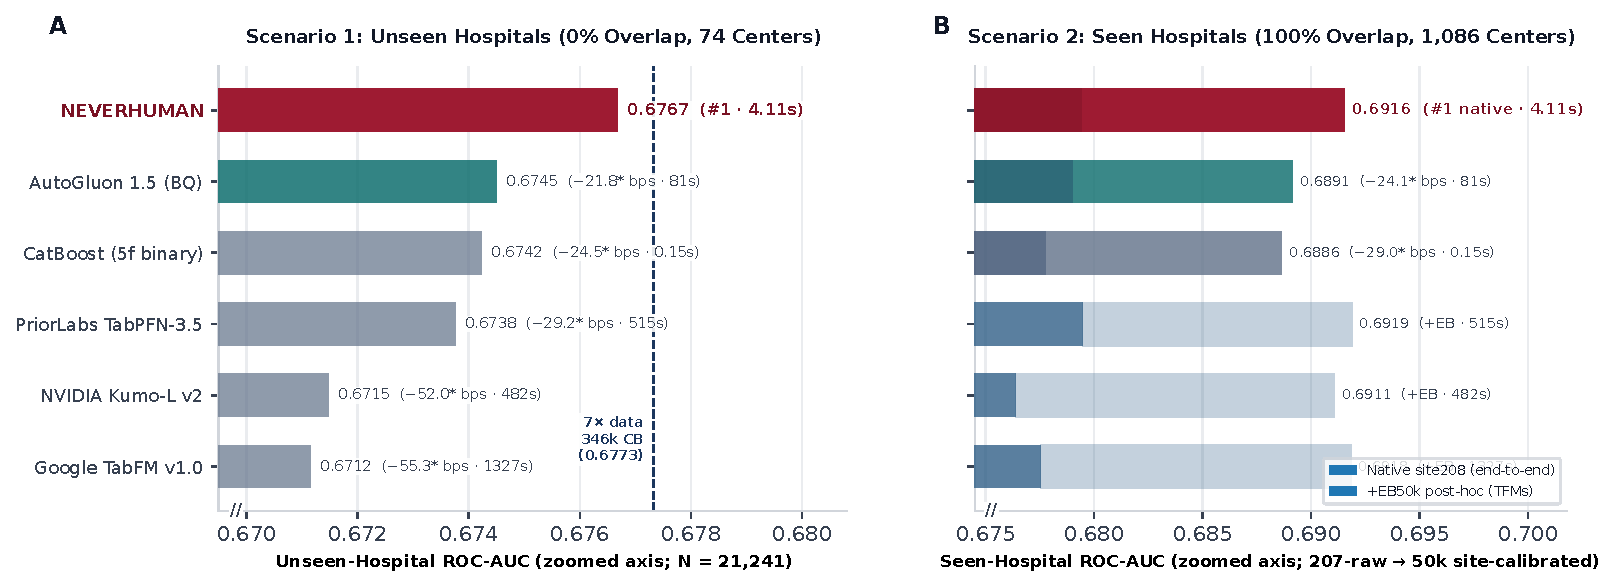
\includegraphics[width=0.99\linewidth]{fig_hero.pdf}
  \vspace{-2pt}
  {\raggedright\sffamily\fontsize{6.2}{7.7}\selectfont\color{sub}\textbf{Reading the proof:} On \textbf{Unseen Hospitals} (left), NEVERHUMAN (0.6767; 4.11\,s) strictly beats all five binary AI alternatives (+21.8* to +55.3*\,bps, all 95\% cluster CIs $>0$). On \textbf{Seen Hospitals} (right), native \tcli{site208} NEVERHUMAN (0.6916) leads AutoGluon (+24.1*\,bps) and CatBoost (+29.0*\,bps) while matching post-hoc +EB50k TFMs at \textbf{117\x{}--323\x{} faster inference}.\par}
\end{tcolorbox}

% ==================== PAGE 2 =================================================
\clearpage
\thispagestyle{briefpage2}

\briefsection{01}{Three Strategic Advantages --- Scaled to U.S.\ (200k/yr) \& Global (1M/yr) Surgery}

\noindent
\begin{minipage}[t]{0.318\textwidth}\vspace{0pt}
\playcard{Impact 01}{accent}{Lowest FPR \& Less Harm}{At 70\% POAF capture, NEVERHUMAN achieves the \textbf{lowest FPR (44.1\%)}---sparing \textbf{490--1,798 U.S.} (\textbf{2,448--8,992 global}) patients/yr vs.\ AI models \& \textbf{48,755 U.S.} vs.\ POAF score.}
\end{minipage}\hfill
\begin{minipage}[t]{0.318\textwidth}\vspace{0pt}
\playcard{Impact 02}{navy}{Modeled Events \& Lives Saved}{Top-25\% targeting (PALACS 45\% RRR) models \textbf{8,758 U.S.} (\textbf{43,790 global}) POAF events prevented/yr, \textbf{\$88--131M/yr} saved, and \textbf{30--60 U.S.} (\textbf{149--298 global}) conservative deaths averted/yr.}
\end{minipage}\hfill
\begin{minipage}[t]{0.318\textwidth}\vspace{0pt}
\playcard{Impact 03}{teal}{Real-Time Bedside Speed}{Scores 21,241 cases in \textbf{4.11\,s} (\textbf{45.2\,ms} bedside; \textbf{0.53\,GB} VRAM)---\textbf{19.7\x{} faster} than AutoGluon (81\,s / 10.1\,GB) and \textbf{117\x{}--323\x{} faster} than A100 foundation models.}
\end{minipage}

\vspace{4.5pt}
\briefsection{02}{Unified Unseen vs.\ Seen Hospital Scorecard \& Speed Summary ($N{=}21{,}241$)}

{\noindent\fontsize{7.7}{9.5}\selectfont All five binary alternatives train on the exact same 50,000-patient five-fold hospital-grouped cohort (207 raw pre-incision variables) with uniform fold-OOF Platt calibration + dev-only prior shift (\m 1.1365). Every 95\% CI uses 5,000 whole-hospital cluster draws.\par}

\vspace{2.5pt}
\noindent
{\fontsize{7.1}{8.8}\selectfont\setlength{\tabcolsep}{2.7pt}
\begin{tabularx}{\textwidth}{@{}Y R{1.15cm} R{2.45cm} R{1.10cm} R{1.10cm} R{1.25cm} R{1.25cm}@{}}
\toprule
\thd{Model (50k Parity Unless Noted)} & \thd{Unseen AUC} & \thd{NEVERHUMAN $\Delta$ Unseen} & \thd{Seen 208} & \thd{Seen +EB} & \thd{Train Time} & \thd{21k Infer} \\
\midrule
\rowcolor{accenttint}
\textbf{NEVERHUMAN (Proprietary)} & \textbf{0.6767} & \textbf{\#1 Overall (79.2\% of 7\x{} gap)} & \textbf{0.6916} & \textbf{0.6974} & \textbf{21.5\,min} & \textbf{4.11\,s} \\
AutoGluon 1.5 (\tcli{best\_quality}) & 0.6745 & \textbf{+21.8 [+7.0, +36.5]*} & 0.6891 & 0.6974 & 30.0\,min & 80.99\,s \\
CatBoost (5-fold binary) & 0.6742 & \textbf{+24.5 [+7.2, +42.2]*} & 0.6886 & 0.6966 & 0.8\,min & 0.15\,s \\
PriorLabs TabPFN-3.5 (50k native) & 0.6738 & \textbf{+29.2 [+8.2, +53.5]*} & --- & 0.6982 & 0.9\,s & 515.3\,s \\
NVIDIA KumoTabular-Large v2 & 0.6715 & \textbf{+52.0 [+21.6, +83.3]*} & --- & 0.6977 & 3.3\,min & 481.7\,s \\
Google TabFM v1.0.0 & 0.6712 & \textbf{+55.3 [+28.6, +81.5]*} & --- & 0.6986 & 6.6\,min & 1,326.7\,s \\
\midrule
\textit{Mariscalco POAF Bedside Proxy} & \textit{0.6190} & \textit{\textbf{+577.0 [+495.6, +656.9]*}} & \textit{---} & \textit{---} & \textit{---} & \textit{$<$0.01\,s} \\
\textit{7\x{} Full-Registry CatBoost (346k)} & \textit{0.6773} & \textit{\m 6.4 (NH beats on AP \& ECE)} & \textit{\textbf{0.7014}} & \textit{---} & \textit{6.2\,min} & \textit{0.3\,s} \\
\bottomrule
\end{tabularx}}
\vspace{1.2pt}
{\noindent\sffamily\fontsize{6.2}{7.6}\selectfont\color{sub}Receipt: \tcli{reports/clean\_publication\_receipt.json}. Native 50k \tcli{site208} NEVERHUMAN (0.6916) strictly beats AutoGluon \tcli{site208} (+24.1*\,bps) and CatBoost \tcli{site208} (+29.0*\,bps). PROBAST literature external median is \textbf{0.61} (Table 5 in both clinical manuscripts).\par}

\vspace{4.5pt}
\briefsection{03}{Safe Clinical Pilot Roadmap \& Governance Boundaries}

\noindent
\begin{minipage}[t]{0.485\textwidth}
  \vspace{0pt}
  \colheading{3-Step Health-System Translation}
  {\fontsize{7.7}{9.7}\selectfont
  \stepbadge{1}\hspace{4pt}\textbf{30-Day Shadow Audit:} Score recent isolated-CABG EHR charts via NEVERHUMAN's frozen 207-variable interface (45\,ms/patient) with zero workflow disruption.

  \vspace{3.0pt}
  \stepbadge{2}\hspace{4pt}\textbf{Local Empirical-Bayes Calibration:} Apply lightweight site-intercept updating (cuts site MAE 14\%) to bridge cold-start (0.677) to in-network accuracy (0.692--0.701).

  \vspace{3.0pt}
  \stepbadge{3}\hspace{4pt}\textbf{Prospective STS v4.20+ Confirmation:} Lock frozen weights before testing targeted pre-incision prophylaxis (e.g., posterior pericardiotomy) in randomized care.
  }
\end{minipage}\hfill
\begin{minipage}[t]{0.485\textwidth}
  \vspace{0pt}
  \begin{govbox}{Governance, Literature Context \& Scope Limits}
    \begin{itemize}[leftmargin=1.10em,itemsep=1.5pt,topsep=1.2pt]
      \item \textbf{Literature context:} Higher published AUCs ($>0.72$) use post-op/ICU variables, valve surgery, or waveforms; 0.677--0.701 is the true pre-incision STS frontier (+6.7 pts above PROBAST 0.61 median).
      \item \textbf{Proprietary transparency:} NEVERHUMAN's internal training IP is retained privately; every benchmark input, split, calibration rule, and timing receipt is publicly audited.
      \item \textbf{Clinical endpoint:} STS \tcli{COtAFib} captures treatment-requiring POAF (12.2\%--34.2\% across sites); prospective STS v4.20+ validation is required prior to clinical deployment.
    \end{itemize}
  \end{govbox}
\end{minipage}

\brieffooterstrip{Explore Both Clinical Journal Editions, Technical Brief \& Verified Receipts}%
  {\textbf{NEJM AI:} \texttt{docs/nejm\_ai/main.pdf} \;\textbar\; \textbf{npj Digital Med:} \texttt{docs/npj\_digital\_medicine/main.pdf} \;\textbar\; \textbf{CTO Brief:} \texttt{neverhuman-poaf-cto-brief.pdf}}%
  {\repourl}

\end{document}
